\section{Comparador de magnitud \label{sec:s2}}

\begin{center}
	\begin{minipage}{12cm}
		\begin{tcolorbox}[title=Actividad 2]
			Completar el código del comparador de magnitud en el lenguaje de su elección, para entradas de 4 bits. Compilar y simular. Configurar en la tarjeta DE2-115, asignar interruptores como entradas y un LED para observar la salida.
		\end{tcolorbox}	
	\end{minipage}
\end{center}

La visualización RTL del comparador de magnitud en Verilog se muestra en la \autoref{fig:magnitude_comparator_rtl}. Como se observa, la implementación del comparador de magnitud se hace utilizando un comparador de igualdad que pone la salida en alto unicamente cuando ambas entradas tienen el mismo valor. Las simulaciones para el código en Verilog se visualizan en la \autoref{fig:magnitude_comparator_WaveBi} en base binaria y en la \autoref{fig:magnitude_comparator_WaveDe} en base decimal. Se utilizaron todos los valores posibles en las entradas para observar un comportamiento completo en la salida.

\begin{figure}[ht]
	\centering
	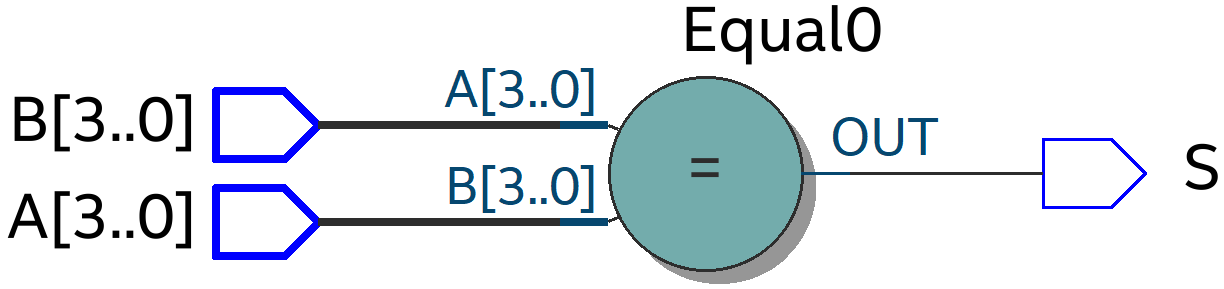
\includegraphics[scale=0.5]{Magnitude_Comparator_RTL.png}
	\caption{Diagrama RTL del comparador de magnitud. \label{fig:magnitude_comparator_rtl}}
\end{figure}

\begin{figure}[ht]
	\centering
	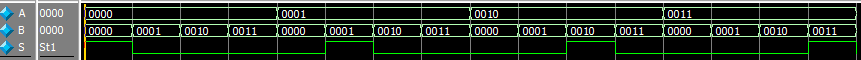
\includegraphics[scale=0.75]{Magnitude_Comparator_WaveBi.png}
	\caption{Simulación del comparador de magnitud con el visor de formas de onda de ModelSim (Base binaria). \label{fig:magnitude_comparator_WaveBi}}
\end{figure}

\begin{figure}[ht]
	\centering
	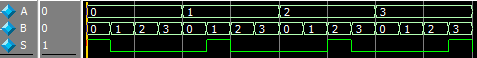
\includegraphics[scale=1.3]{Magnitude_Comparator_WaveDe.png}
	\caption{Simulación del comparador de magnitud con el visor de formas de onda de ModelSim (Base decimal). \label{fig:magnitude_comparator_WaveDe}}
\end{figure}





